% So we make this "beamer" rather than document!

\documentclass[11pt]{beamer}
\usetheme[sectionpage=none, numbering=none]{metropolis}           % Use metropolis theme
	% Kill page numbers with [numbering=none] in next line:
	% To do printouts, add ", handout"  after aspectratio.
\usepackage{makecell}
\usepackage{booktabs}
%\usepackage{graphicx}
\usepackage{color}
%\usepackage[utf-8]{inputenc}
\usepackage{minted}


\title{Julia \\ \emph{Feels like Python; Works like Lisp; Fast like C}}
\author{	\small Nick Eubank \\
			\scriptsize{CSDI, Vanderbilt University}\vspace*{.15in} \\}
\date{\vspace*{.3in} \today}



% Problem:
%   Forced choice
%   Lead to two language problem
%   Makes hard to
%       - Understand inner workings
%       - Modify libraries
%       - Write new libraries
%   Julia aims to solve
%

%

% This is the beginning of a real document!
\begin{document}


\begin{frame}
	\maketitle
\end{frame}

\begin{frame}[c]{Who am I?}
\begin{itemize}
    \item Post-Doc at Center for Study of Democratic Institutions
    \item Study social networks using cell-phone meta-data
    \begin{itemize}
        \item Lots of simulations on networks with $>$10,000,000 nodes
    \end{itemize}
    \item Regularly work with Stata, R, Python, and Julia
    \begin{itemize}
        \item Some contributions to Julia packages, but I am \emph{not} a core Julia developer!
    \end{itemize}
\end{itemize}
\end{frame}

\begin{frame}{}
\centering
\pause
    \begin{minipage}[t]{0.48\linewidth}
        Easy To Use Languages\\
        \emph{Python, R, Matlab}
        \begin{itemize}
            \item<3-> Interactive
            \item<4-> Dynamic typed
            \item<5-> Fast to write
            \item<6-> Slow to run
        \end{itemize}
    \end{minipage}
    \vrule{}
    \begin{minipage}[t]{0.48\linewidth}%
        Fast Languages\\
        \emph{C, Java}
        \begin{itemize}
            \item<3-> Compiled
            \item<4-> Static Typed
            \item<5-> Slow to write
            \item<6-> Fast to run
        \end{itemize}
    \end{minipage}
\end{frame}

\begin{frame}[c]{}
\begin{itemize}
    \item Write core libraries in C or Fortran
    \item Wrap in a nice language (R or Python)
\end{itemize}
\end{frame}

\begin{frame}[c]{Two Language Problem}
\begin{itemize}
    \pause \item Hard to \alert{understand} workings of packages
    \pause \item Hard to \alert{modify} packages
    \pause \item Hard to \alert{write} performant packages
\end{itemize}
\pause
\vspace*{1cm}
$\Rightarrow$ True if you know C... \\
\pause $\Rightarrow$ \emph{Extremely} true if you don't know C!
\end{frame}

\begin{frame}[c]{No Two Language Problem}
Base Julia is written \emph{in Julia}
\begin{itemize}
    \item Even things like definitions of integers!
\end{itemize}
Most packages written in pure Julia
\end{frame}

\begin{frame}[fragile, t]{}
\begin{minted}[fontsize=\small]{python}
# Python
def sum_sequence(start, stop):
    total = 0
    for i in range(start, stop):
        total = total + i
    return total
\end{minted}
\begin{minted}[fontsize=\small]{julia}
# Julia
function sum_sequence(start, stop)
    total = 0
    for i in start:stop
        total = total + i
    end
    return total
end
    \end{minted}
\pause
Python: \texttt{sum\_sequence(0, 1000000)}: 78.8 milliseconds\\
Julia: \texttt{sum\_sequence(0, 1\_000\_000)}: 0.0037 milliseconds
\end{frame}

\begin{frame}[c]{}
    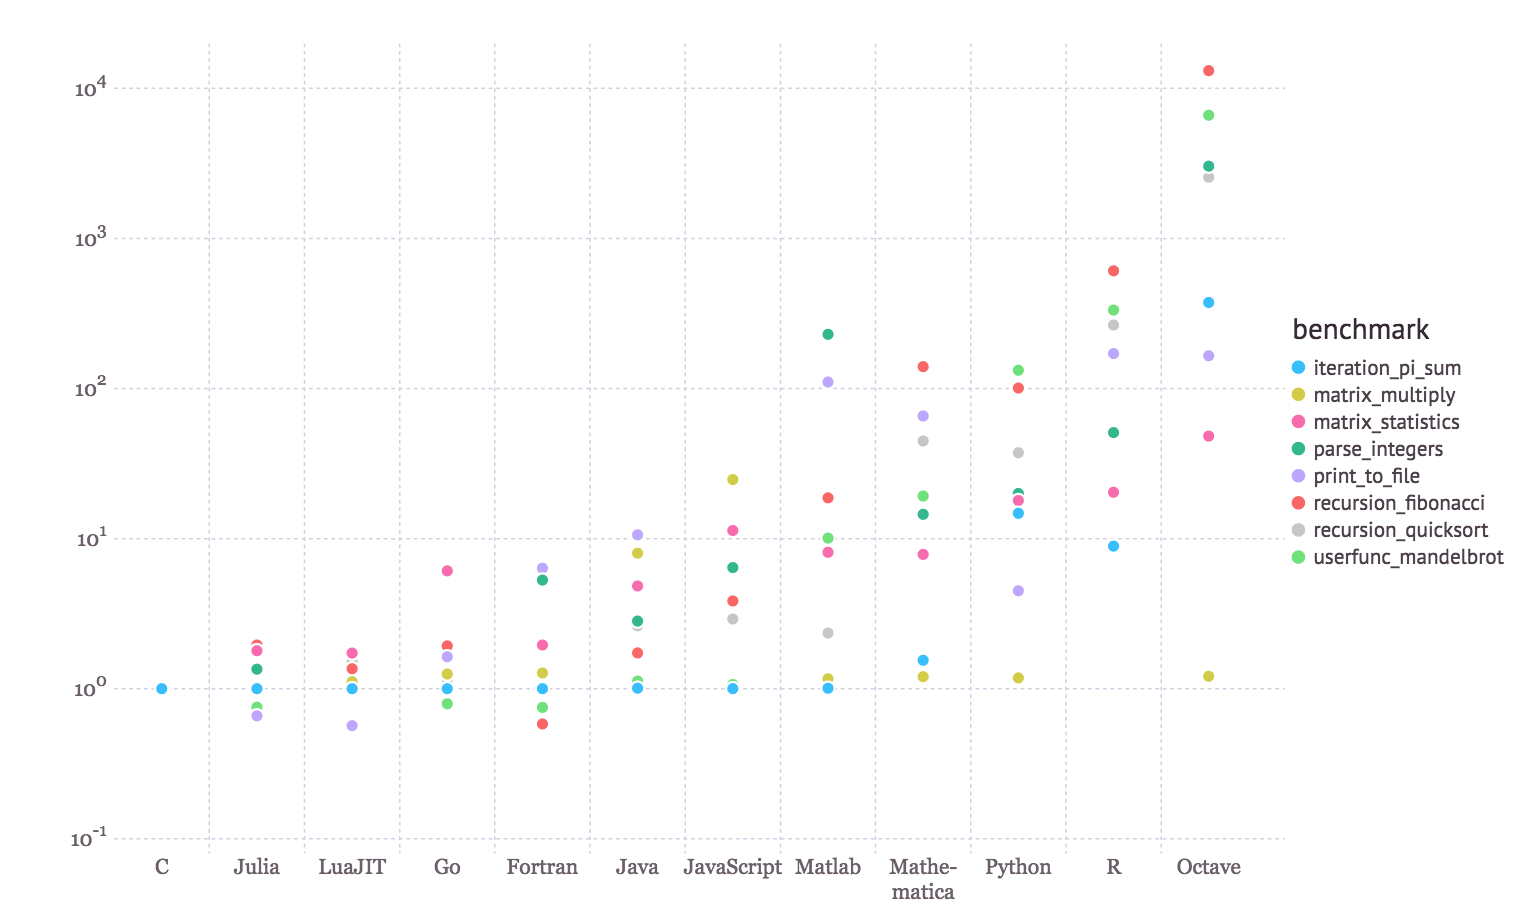
\includegraphics[width=\textwidth]{figures/benchmarks.png}
\end{frame}


\begin{frame}[fragile, t]{Why Python (and R) are slow }
\begin{minted}{python}
# Python
def sum_sequence(0, 1000000):
    total = 0
    for i in range(start, stop):
        total = total + i
    return total
\end{minted}
\pause
\begin{itemize}
    \item Your processor doesn't know what ``add total and i'' means...
    \begin{itemize}
        \pause \item Not all numbers are created equal
        \pause \item \texttt{+} actually has different meanings
    \end{itemize}
\end{itemize}
\pause
$\Rightarrow$Checks type of \texttt{total}, type of \texttt{i}, and looks up appropriate function \texttt{+} one million times!
\end{frame}

\begin{frame}[fragile, t]{Why Julia is Fast}
\begin{minted}{julia}
# Julia
function sum_sequence(start, stop)
    total = 0
    for i in start:stop
        total = total + i
    end
    return total
end
    \end{minted}
\begin{itemize}
    \pause \item  Treats function as a small program.
    \pause \item Realizes that \texttt{total} and \texttt{i} are always going to be integers, so only checks once.
    \pause \item Keeps copy of machine code once created so doesn't have to re-evaluate every time function is called.
\end{itemize}
\end{frame}

\begin{frame}[fragile]{Corollary: Julia is only fast inside functions}
\begin{minted}[fontsize=\small]{julia}
# Slow
total = 0
for i in 0:1_000_000
    total = total + i
end
\end{minted}
\pause
\begin{minted}[fontsize=\small]{julia}
# Fast
function sum_sequence(start, stop)
    total = 0
    for i in start:stop
        total = total + i
    end
    return total
end
sum_sequence(0, 1_000_000)
\end{minted}
\end{frame}


\begin{frame}[fragile]{Features: Just Write the Loop}
\begin{itemize}
    \item No more need to always vectorize!
    \item But if you want, you still can with \texttt{.} notation.
\end{itemize}
\begin{minted}{julia}
x = rand(100)

# Loop
for i in 1:length(x)
    x[i] = sqrt(x[i])
end

# Vectorized
x = sqrt.(x)
\end{minted}
Times: 6.651 ms (loop) and 7.682 ms (vectorized)
\end{frame}

\begin{frame}[fragile]{Features: Native Parallelism}
Add workers:
\begin{minted}{julia}
addprocs(3)
\end{minted}
Small jobs:
\begin{minted}{julia}
num_heads = @parallel (+) for i in 1:1_000_000
                rand(Bool)
            end
\end{minted}
Or:
\begin{minted}{julia}
a = SharedArray{Float64}(1_000)
@parallel for i = 1:1_000
    a[i] = randn()
end
\end{minted}
\end{frame}


\begin{frame}[fragile]{Features: Parallelism}
Big jobs:
\begin{minted}{julia}
svds = pmap(svd, list_of_matrices)
\end{minted}
\end{frame}

\begin{frame}[fragile]{Features: Support for Unicode}
OLS with Unicode:
\begin{minted}{julia}
N = 4000
x = randn(N, 3)
ϵ = randn(N)
β = [2, 1, 90]
y = x * β + ϵ

β̂ = inv(x' * x) * x' * y
ϵ̂ = y - x * β̂
\end{minted}
\end{frame}



\begin{frame}[fragile]{Features: Easy C Integration}
If you need it, use \texttt{ccall}.
\pause
Here's a call to \texttt{clock} function in C library \texttt{libc} that takes no arguments and returns an \texttt{Int32} value:
\begin{minted}{julia}
t = ccall((:clock, "libc"), Int32, ())
\end{minted}
\end{frame}

\begin{frame}[fragile]{Features: Easy Python Integration}
Import python \texttt{math} function and use its functions in Julia.
\begin{minted}{julia}
using PyCall
@pyimport math
math.sin(math.pi / 4) - sin(pi / 4)
\end{minted}
\end{frame}


\begin{frame}[c]{Not 1.0 Yet...}
Currently Stable Release: 0.6.2
Pending Release: 0.7
\begin{itemize}
    \item Expected this summer ($\sim$ June 2018?)
    \item 0.7 is 1.0 with depreciation warnings
    \begin{itemize}
        \item If you code works with 0.7, syntax won't change!
    \end{itemize}
\end{itemize}
\end{frame}

\begin{frame}[c]{Expected changes}
\begin{itemize}
    \pause \item Major compiler improvements for missing data
    \pause \item New package manager
    \pause \item Missing data type moving to core library
\end{itemize}
\end{frame}

\begin{frame}[c]{Hands-on Tutorials!}
    Go to \url{juliabox.com}, create an account, and navigate to \texttt{tutorials/intro-to-julia}.
\end{frame}

\begin{frame}[c]{Resources}
    Comparing Julia, Python, and Matlab side by side: \\
    \url{https://cheatsheets.quantecon.org/} \\
    Amazing cheatsheet for Julia: \\
    \url{https://juliadocs.github.io/Julia-Cheat-Sheet/}
\end{frame}


\end{document}
